% Options for packages loaded elsewhere
\PassOptionsToPackage{unicode}{hyperref}
\PassOptionsToPackage{hyphens}{url}
\PassOptionsToPackage{dvipsnames,svgnames,x11names}{xcolor}
%
\documentclass[
]{apa7}

\usepackage{amsmath,amssymb}
\usepackage{iftex}
\ifPDFTeX
  \usepackage[T1]{fontenc}
  \usepackage[utf8]{inputenc}
  \usepackage{textcomp} % provide euro and other symbols
\else % if luatex or xetex
  \usepackage{unicode-math}
  \defaultfontfeatures{Scale=MatchLowercase}
  \defaultfontfeatures[\rmfamily]{Ligatures=TeX,Scale=1}
\fi
\usepackage{lmodern}
\ifPDFTeX\else  
    % xetex/luatex font selection
\fi
% Use upquote if available, for straight quotes in verbatim environments
\IfFileExists{upquote.sty}{\usepackage{upquote}}{}
\IfFileExists{microtype.sty}{% use microtype if available
  \usepackage[]{microtype}
  \UseMicrotypeSet[protrusion]{basicmath} % disable protrusion for tt fonts
}{}
\makeatletter
\@ifundefined{KOMAClassName}{% if non-KOMA class
  \IfFileExists{parskip.sty}{%
    \usepackage{parskip}
  }{% else
    \setlength{\parindent}{0pt}
    \setlength{\parskip}{6pt plus 2pt minus 1pt}}
}{% if KOMA class
  \KOMAoptions{parskip=half}}
\makeatother
\usepackage{xcolor}
\setlength{\emergencystretch}{3em} % prevent overfull lines
\setcounter{secnumdepth}{-\maxdimen} % remove section numbering
% Make \paragraph and \subparagraph free-standing
\makeatletter
\ifx\paragraph\undefined\else
  \let\oldparagraph\paragraph
  \renewcommand{\paragraph}{
    \@ifstar
      \xxxParagraphStar
      \xxxParagraphNoStar
  }
  \newcommand{\xxxParagraphStar}[1]{\oldparagraph*{#1}\mbox{}}
  \newcommand{\xxxParagraphNoStar}[1]{\oldparagraph{#1}\mbox{}}
\fi
\ifx\subparagraph\undefined\else
  \let\oldsubparagraph\subparagraph
  \renewcommand{\subparagraph}{
    \@ifstar
      \xxxSubParagraphStar
      \xxxSubParagraphNoStar
  }
  \newcommand{\xxxSubParagraphStar}[1]{\oldsubparagraph*{#1}\mbox{}}
  \newcommand{\xxxSubParagraphNoStar}[1]{\oldsubparagraph{#1}\mbox{}}
\fi
\makeatother

\usepackage{color}
\usepackage{fancyvrb}
\newcommand{\VerbBar}{|}
\newcommand{\VERB}{\Verb[commandchars=\\\{\}]}
\DefineVerbatimEnvironment{Highlighting}{Verbatim}{commandchars=\\\{\}}
% Add ',fontsize=\small' for more characters per line
\usepackage{framed}
\definecolor{shadecolor}{RGB}{241,243,245}
\newenvironment{Shaded}{\begin{snugshade}}{\end{snugshade}}
\newcommand{\AlertTok}[1]{\textcolor[rgb]{0.68,0.00,0.00}{#1}}
\newcommand{\AnnotationTok}[1]{\textcolor[rgb]{0.37,0.37,0.37}{#1}}
\newcommand{\AttributeTok}[1]{\textcolor[rgb]{0.40,0.45,0.13}{#1}}
\newcommand{\BaseNTok}[1]{\textcolor[rgb]{0.68,0.00,0.00}{#1}}
\newcommand{\BuiltInTok}[1]{\textcolor[rgb]{0.00,0.23,0.31}{#1}}
\newcommand{\CharTok}[1]{\textcolor[rgb]{0.13,0.47,0.30}{#1}}
\newcommand{\CommentTok}[1]{\textcolor[rgb]{0.37,0.37,0.37}{#1}}
\newcommand{\CommentVarTok}[1]{\textcolor[rgb]{0.37,0.37,0.37}{\textit{#1}}}
\newcommand{\ConstantTok}[1]{\textcolor[rgb]{0.56,0.35,0.01}{#1}}
\newcommand{\ControlFlowTok}[1]{\textcolor[rgb]{0.00,0.23,0.31}{\textbf{#1}}}
\newcommand{\DataTypeTok}[1]{\textcolor[rgb]{0.68,0.00,0.00}{#1}}
\newcommand{\DecValTok}[1]{\textcolor[rgb]{0.68,0.00,0.00}{#1}}
\newcommand{\DocumentationTok}[1]{\textcolor[rgb]{0.37,0.37,0.37}{\textit{#1}}}
\newcommand{\ErrorTok}[1]{\textcolor[rgb]{0.68,0.00,0.00}{#1}}
\newcommand{\ExtensionTok}[1]{\textcolor[rgb]{0.00,0.23,0.31}{#1}}
\newcommand{\FloatTok}[1]{\textcolor[rgb]{0.68,0.00,0.00}{#1}}
\newcommand{\FunctionTok}[1]{\textcolor[rgb]{0.28,0.35,0.67}{#1}}
\newcommand{\ImportTok}[1]{\textcolor[rgb]{0.00,0.46,0.62}{#1}}
\newcommand{\InformationTok}[1]{\textcolor[rgb]{0.37,0.37,0.37}{#1}}
\newcommand{\KeywordTok}[1]{\textcolor[rgb]{0.00,0.23,0.31}{\textbf{#1}}}
\newcommand{\NormalTok}[1]{\textcolor[rgb]{0.00,0.23,0.31}{#1}}
\newcommand{\OperatorTok}[1]{\textcolor[rgb]{0.37,0.37,0.37}{#1}}
\newcommand{\OtherTok}[1]{\textcolor[rgb]{0.00,0.23,0.31}{#1}}
\newcommand{\PreprocessorTok}[1]{\textcolor[rgb]{0.68,0.00,0.00}{#1}}
\newcommand{\RegionMarkerTok}[1]{\textcolor[rgb]{0.00,0.23,0.31}{#1}}
\newcommand{\SpecialCharTok}[1]{\textcolor[rgb]{0.37,0.37,0.37}{#1}}
\newcommand{\SpecialStringTok}[1]{\textcolor[rgb]{0.13,0.47,0.30}{#1}}
\newcommand{\StringTok}[1]{\textcolor[rgb]{0.13,0.47,0.30}{#1}}
\newcommand{\VariableTok}[1]{\textcolor[rgb]{0.07,0.07,0.07}{#1}}
\newcommand{\VerbatimStringTok}[1]{\textcolor[rgb]{0.13,0.47,0.30}{#1}}
\newcommand{\WarningTok}[1]{\textcolor[rgb]{0.37,0.37,0.37}{\textit{#1}}}

\providecommand{\tightlist}{%
  \setlength{\itemsep}{0pt}\setlength{\parskip}{0pt}}\usepackage{longtable,booktabs,array}
\usepackage{calc} % for calculating minipage widths
% Correct order of tables after \paragraph or \subparagraph
\usepackage{etoolbox}
\makeatletter
\patchcmd\longtable{\par}{\if@noskipsec\mbox{}\fi\par}{}{}
\makeatother
% Allow footnotes in longtable head/foot
\IfFileExists{footnotehyper.sty}{\usepackage{footnotehyper}}{\usepackage{footnote}}
\makesavenoteenv{longtable}
\usepackage{graphicx}
\makeatletter
\newsavebox\pandoc@box
\newcommand*\pandocbounded[1]{% scales image to fit in text height/width
  \sbox\pandoc@box{#1}%
  \Gscale@div\@tempa{\textheight}{\dimexpr\ht\pandoc@box+\dp\pandoc@box\relax}%
  \Gscale@div\@tempb{\linewidth}{\wd\pandoc@box}%
  \ifdim\@tempb\p@<\@tempa\p@\let\@tempa\@tempb\fi% select the smaller of both
  \ifdim\@tempa\p@<\p@\scalebox{\@tempa}{\usebox\pandoc@box}%
  \else\usebox{\pandoc@box}%
  \fi%
}
% Set default figure placement to htbp
\def\fps@figure{htbp}
\makeatother

\usepackage{booktabs}
\usepackage{longtable}
\usepackage{array}
\usepackage{multirow}
\usepackage{wrapfig}
\usepackage{float}
\usepackage{colortbl}
\usepackage{pdflscape}
\usepackage{tabu}
\usepackage{threeparttable}
\usepackage{threeparttablex}
\usepackage[normalem]{ulem}
\usepackage{makecell}
\usepackage{xcolor}
\usepackage{fontspec}
\usepackage{multicol}
\usepackage{hhline}
\newlength\Oldarrayrulewidth
\newlength\Oldtabcolsep
\usepackage{hyperref}
\makeatletter
\@ifpackageloaded{caption}{}{\usepackage{caption}}
\AtBeginDocument{%
\ifdefined\contentsname
  \renewcommand*\contentsname{Table of contents}
\else
  \newcommand\contentsname{Table of contents}
\fi
\ifdefined\listfigurename
  \renewcommand*\listfigurename{List of Figures}
\else
  \newcommand\listfigurename{List of Figures}
\fi
\ifdefined\listtablename
  \renewcommand*\listtablename{List of Tables}
\else
  \newcommand\listtablename{List of Tables}
\fi
\ifdefined\figurename
  \renewcommand*\figurename{Figure}
\else
  \newcommand\figurename{Figure}
\fi
\ifdefined\tablename
  \renewcommand*\tablename{Table}
\else
  \newcommand\tablename{Table}
\fi
}
\@ifpackageloaded{float}{}{\usepackage{float}}
\floatstyle{ruled}
\@ifundefined{c@chapter}{\newfloat{codelisting}{h}{lop}}{\newfloat{codelisting}{h}{lop}[chapter]}
\floatname{codelisting}{Listing}
\newcommand*\listoflistings{\listof{codelisting}{List of Listings}}
\makeatother
\makeatletter
\makeatother
\makeatletter
\@ifpackageloaded{caption}{}{\usepackage{caption}}
\@ifpackageloaded{subcaption}{}{\usepackage{subcaption}}
\makeatother

\usepackage{bookmark}

\IfFileExists{xurl.sty}{\usepackage{xurl}}{} % add URL line breaks if available
\urlstyle{same} % disable monospaced font for URLs
\hypersetup{
  pdftitle={Learn more about Sunny Lee},
  pdfauthor={Sunny Lee},
  colorlinks=true,
  linkcolor={blue},
  filecolor={Maroon},
  citecolor={Blue},
  urlcolor={Blue},
  pdfcreator={LaTeX via pandoc}}


\title{Learn more about Sunny Lee}
\author{Sunny Lee}
\date{}

\begin{document}
\maketitle


\section{Introduction}\label{introduction}

Welcome to my website. This site documents my life as a college student
at UChicago. This is the most authentic and only chance you will get to
learn about the real side of me. Get excited! There will be a brief
overview of my \hyperref[sec-childhood]{childhood},
\hyperref[sec-family-and-friends]{familiy and friends},
\hyperref[sec-student-sunny]{academic passions}, and
\hyperref[sec-other]{other parts of my life}.

\section{Childhood}\label{sec-childhood}

Not invited to analyze my childhood Freudian style, but it helps to
understand what kind of person I am.

\section{Family and friends}\label{sec-family-and-friends}

As a huge extrovert, family and friends are an important part of my
life. People listed on here are my rock and the source of energy in my
life, so\ldots it's a pretty important section.

\begin{figure}[H]

{\centering \pandocbounded{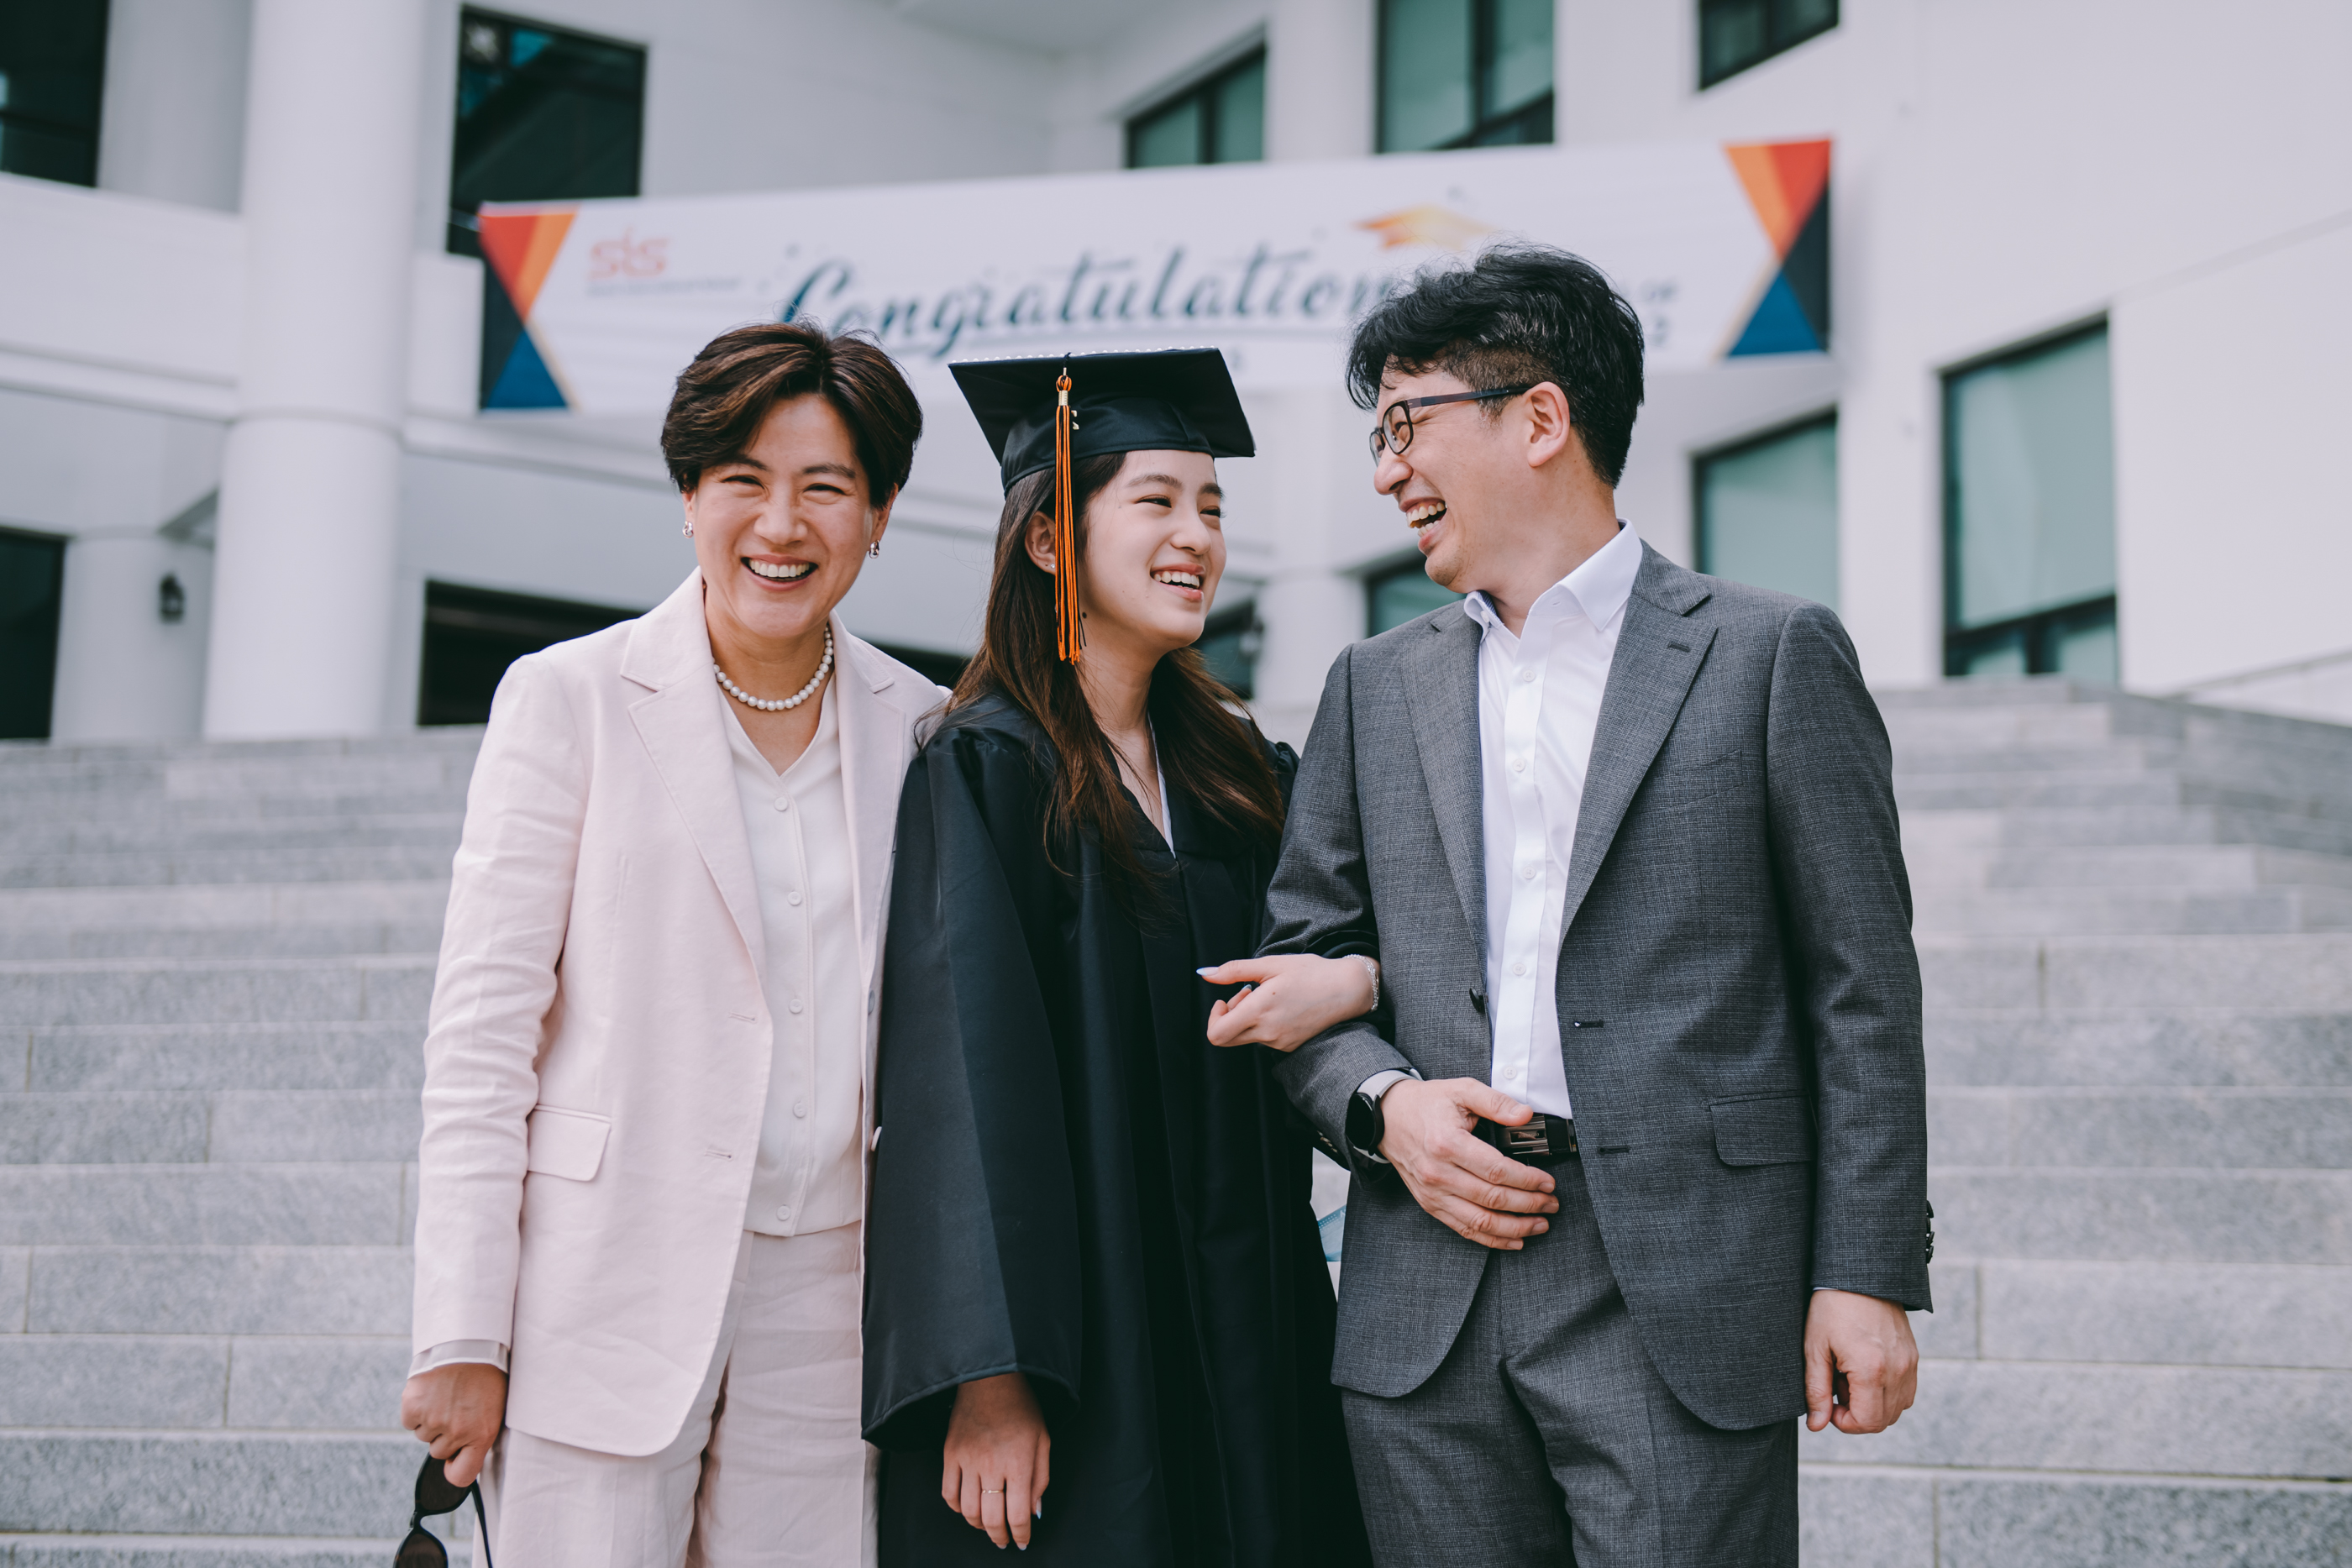
\includegraphics[keepaspectratio]{images/parents.jpg}}

}

\caption{My parents and I at grad}

\end{figure}%

\begin{figure}[H]

{\centering \pandocbounded{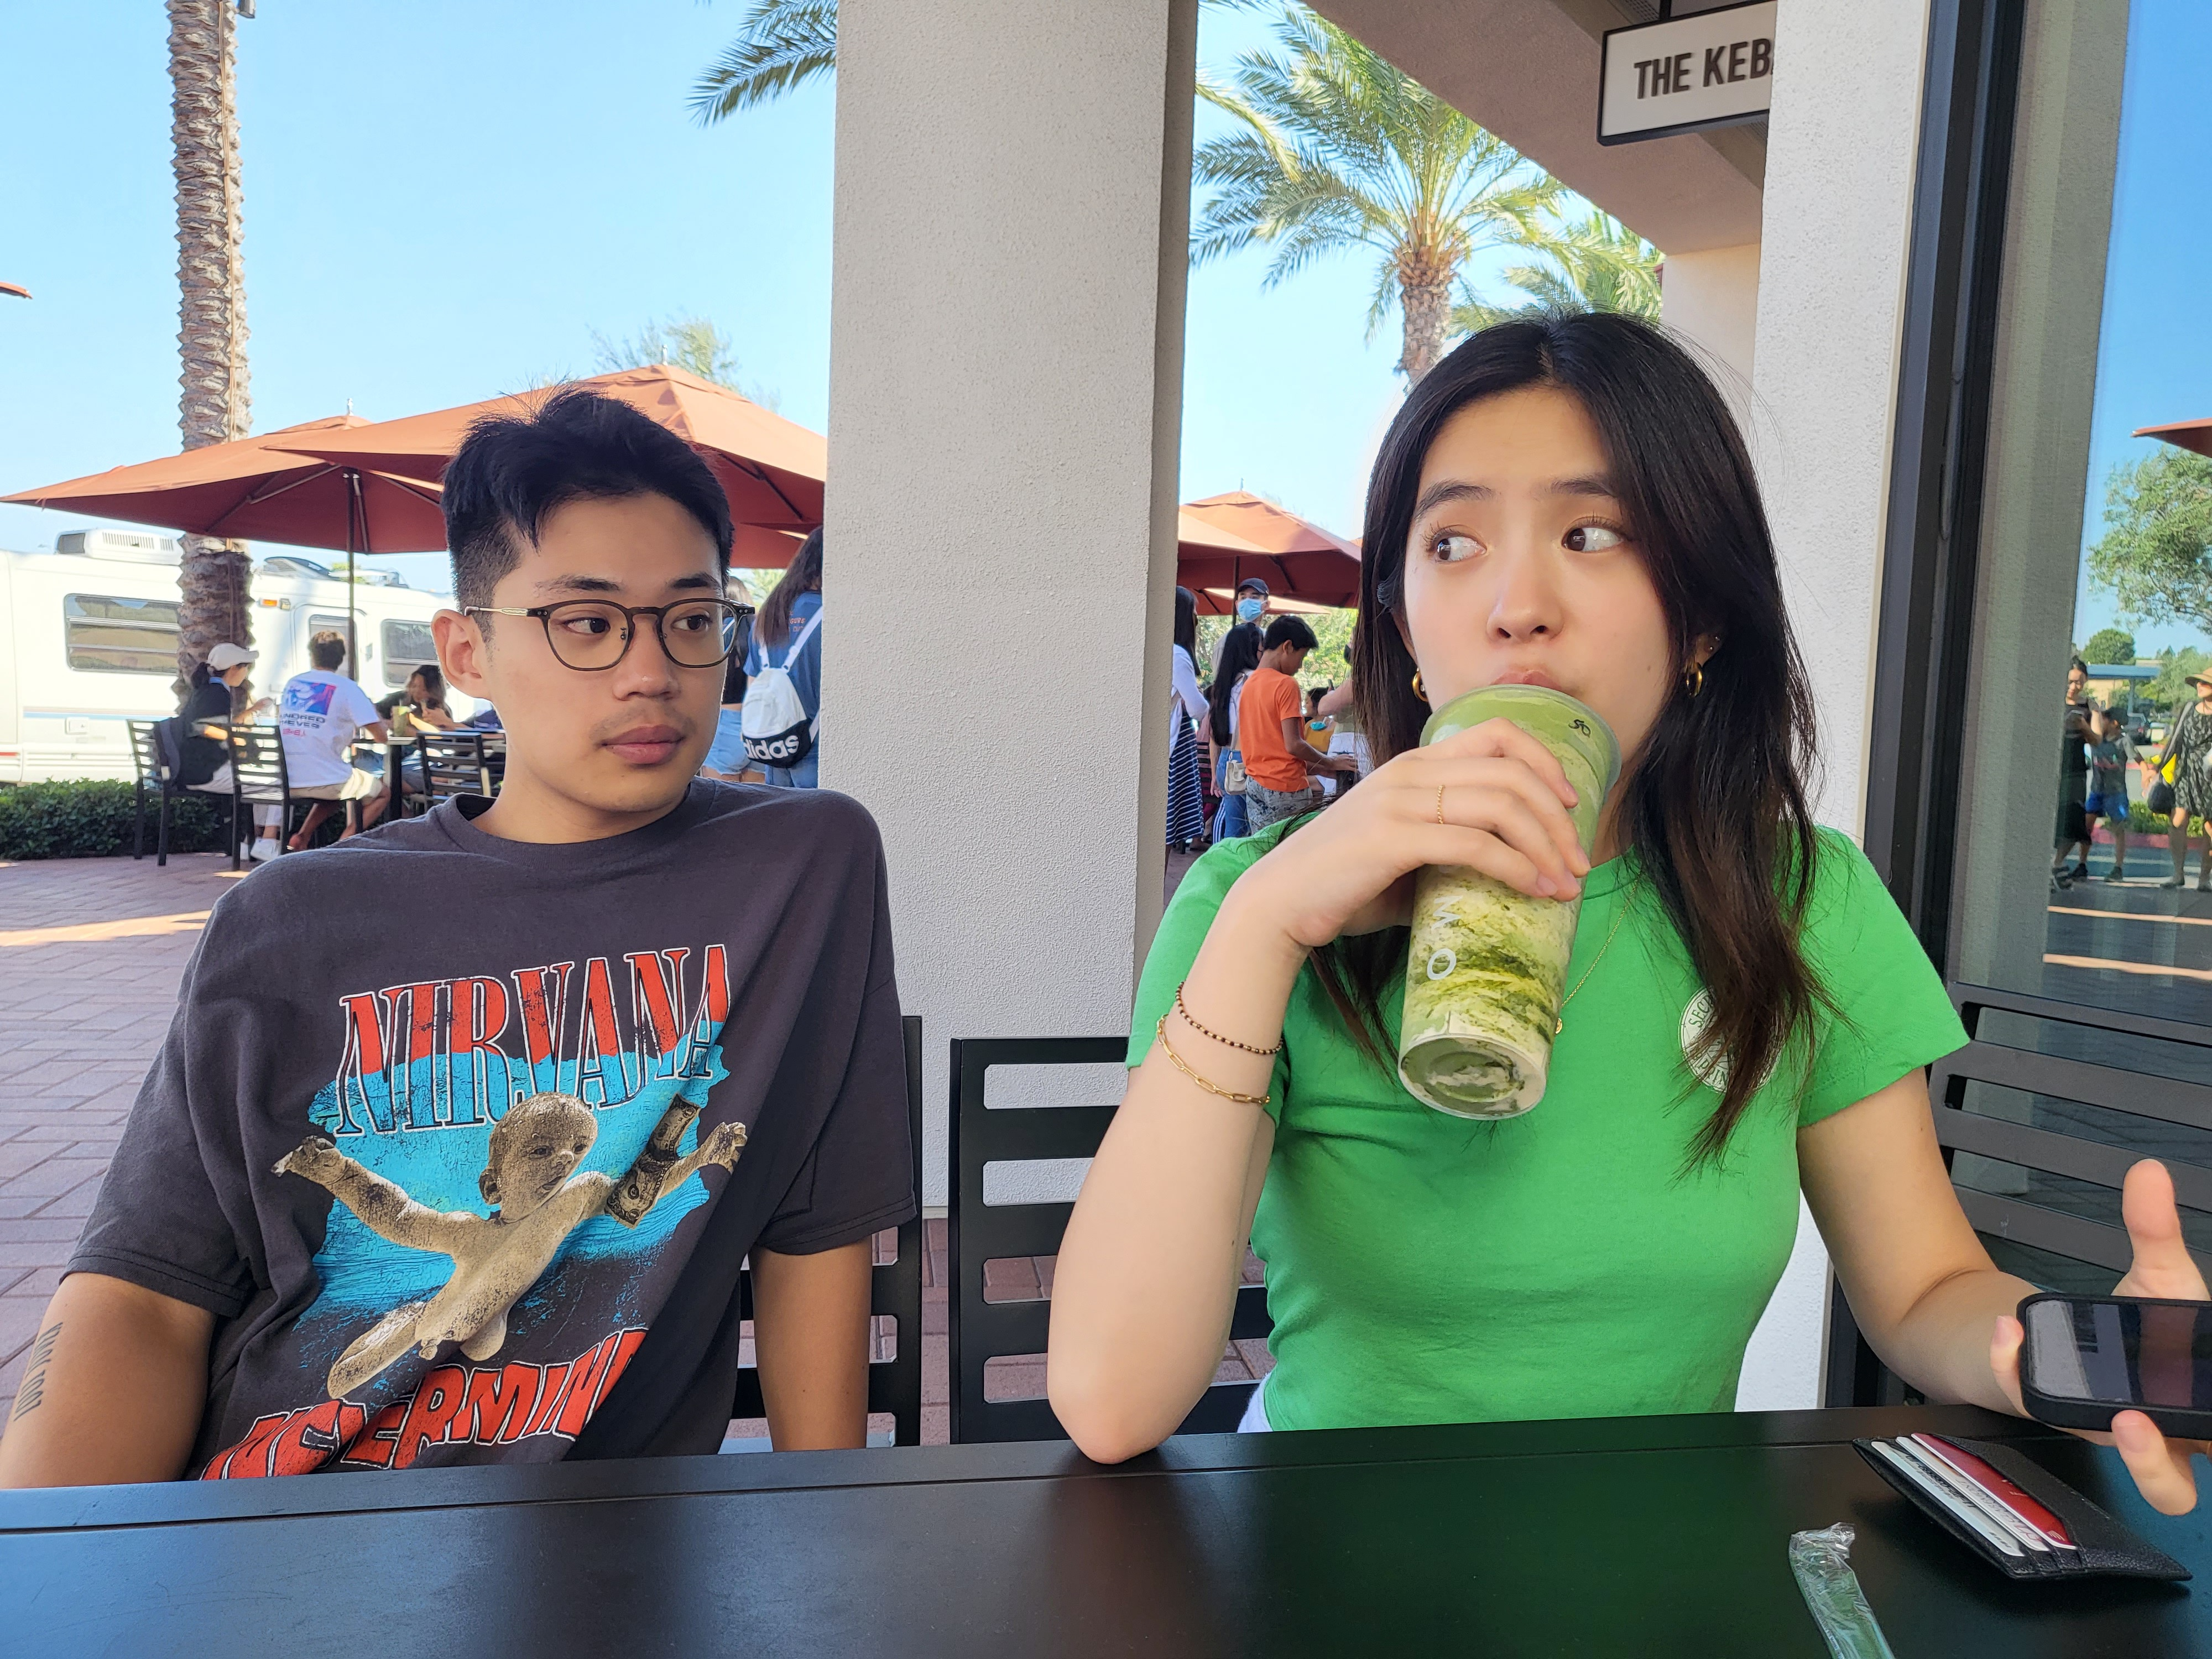
\includegraphics[keepaspectratio]{images/my-brother.JPG}}

}

\caption{At our favorite boba place in Irvine with my brother Ray}

\end{figure}%

\begin{figure}[H]

{\centering \pandocbounded{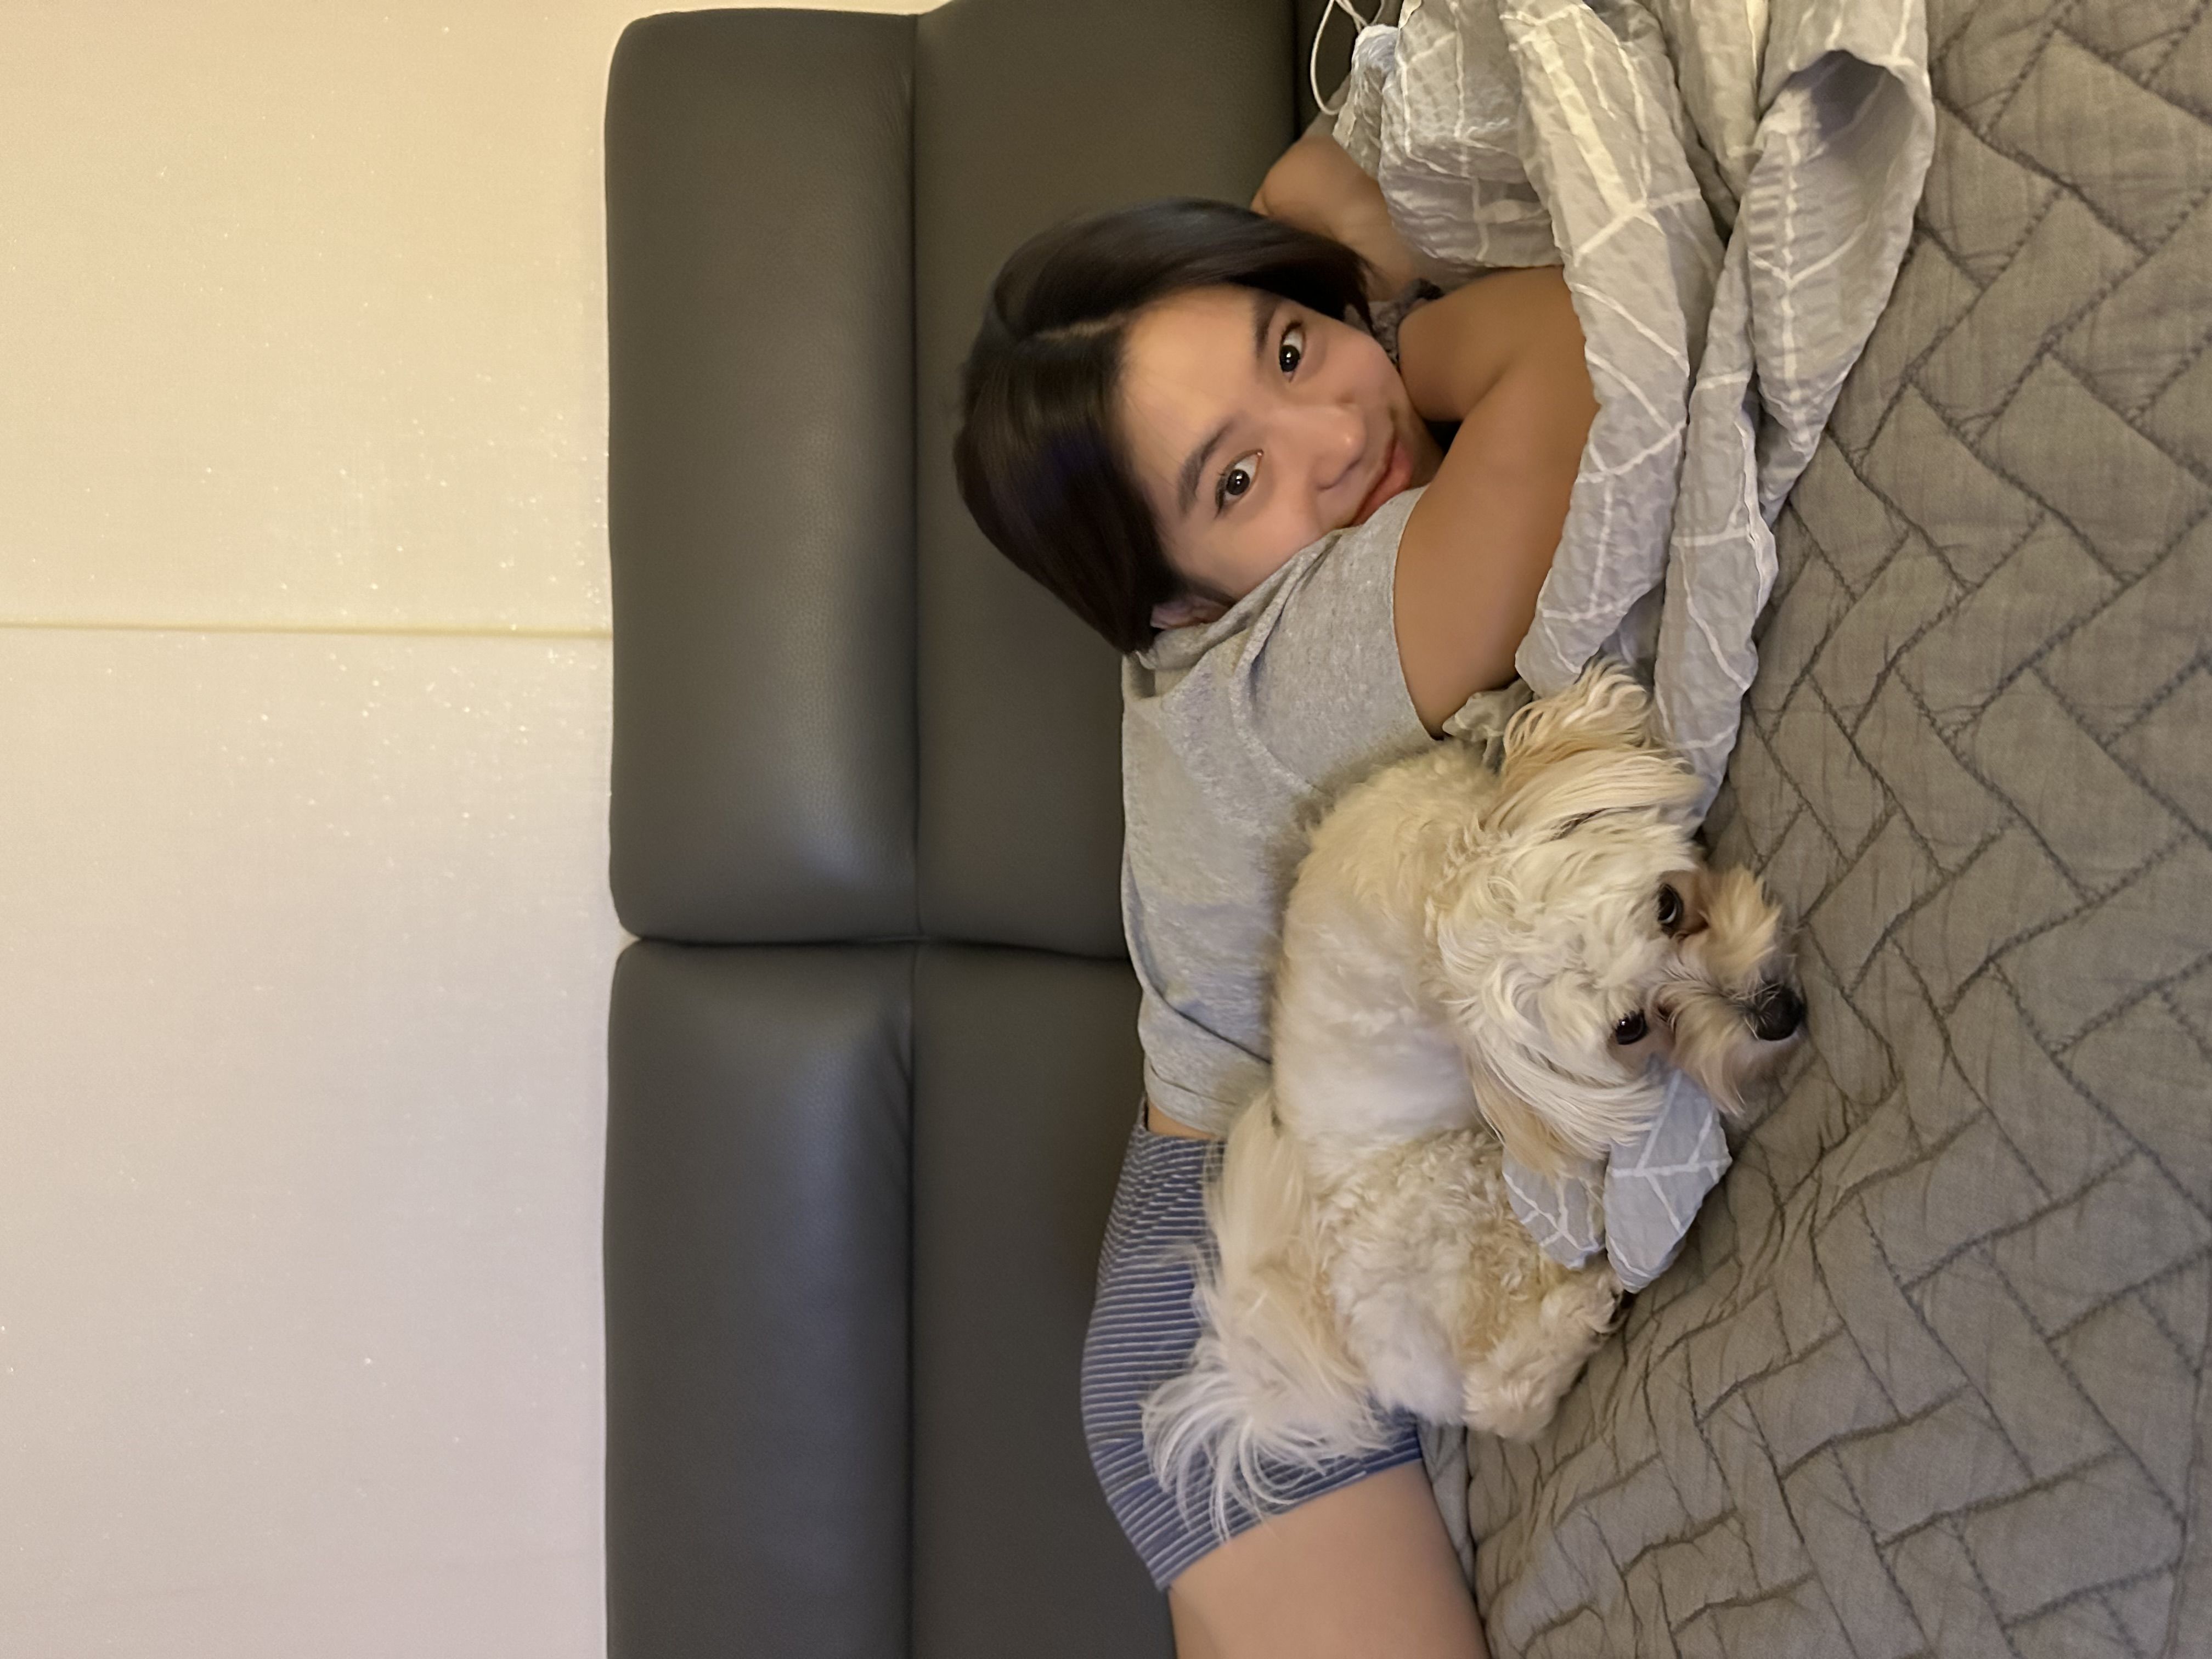
\includegraphics[keepaspectratio]{images/my-dog.jpeg}}

}

\caption{My dog Songyee}

\end{figure}%

\begin{figure}[H]

{\centering \pandocbounded{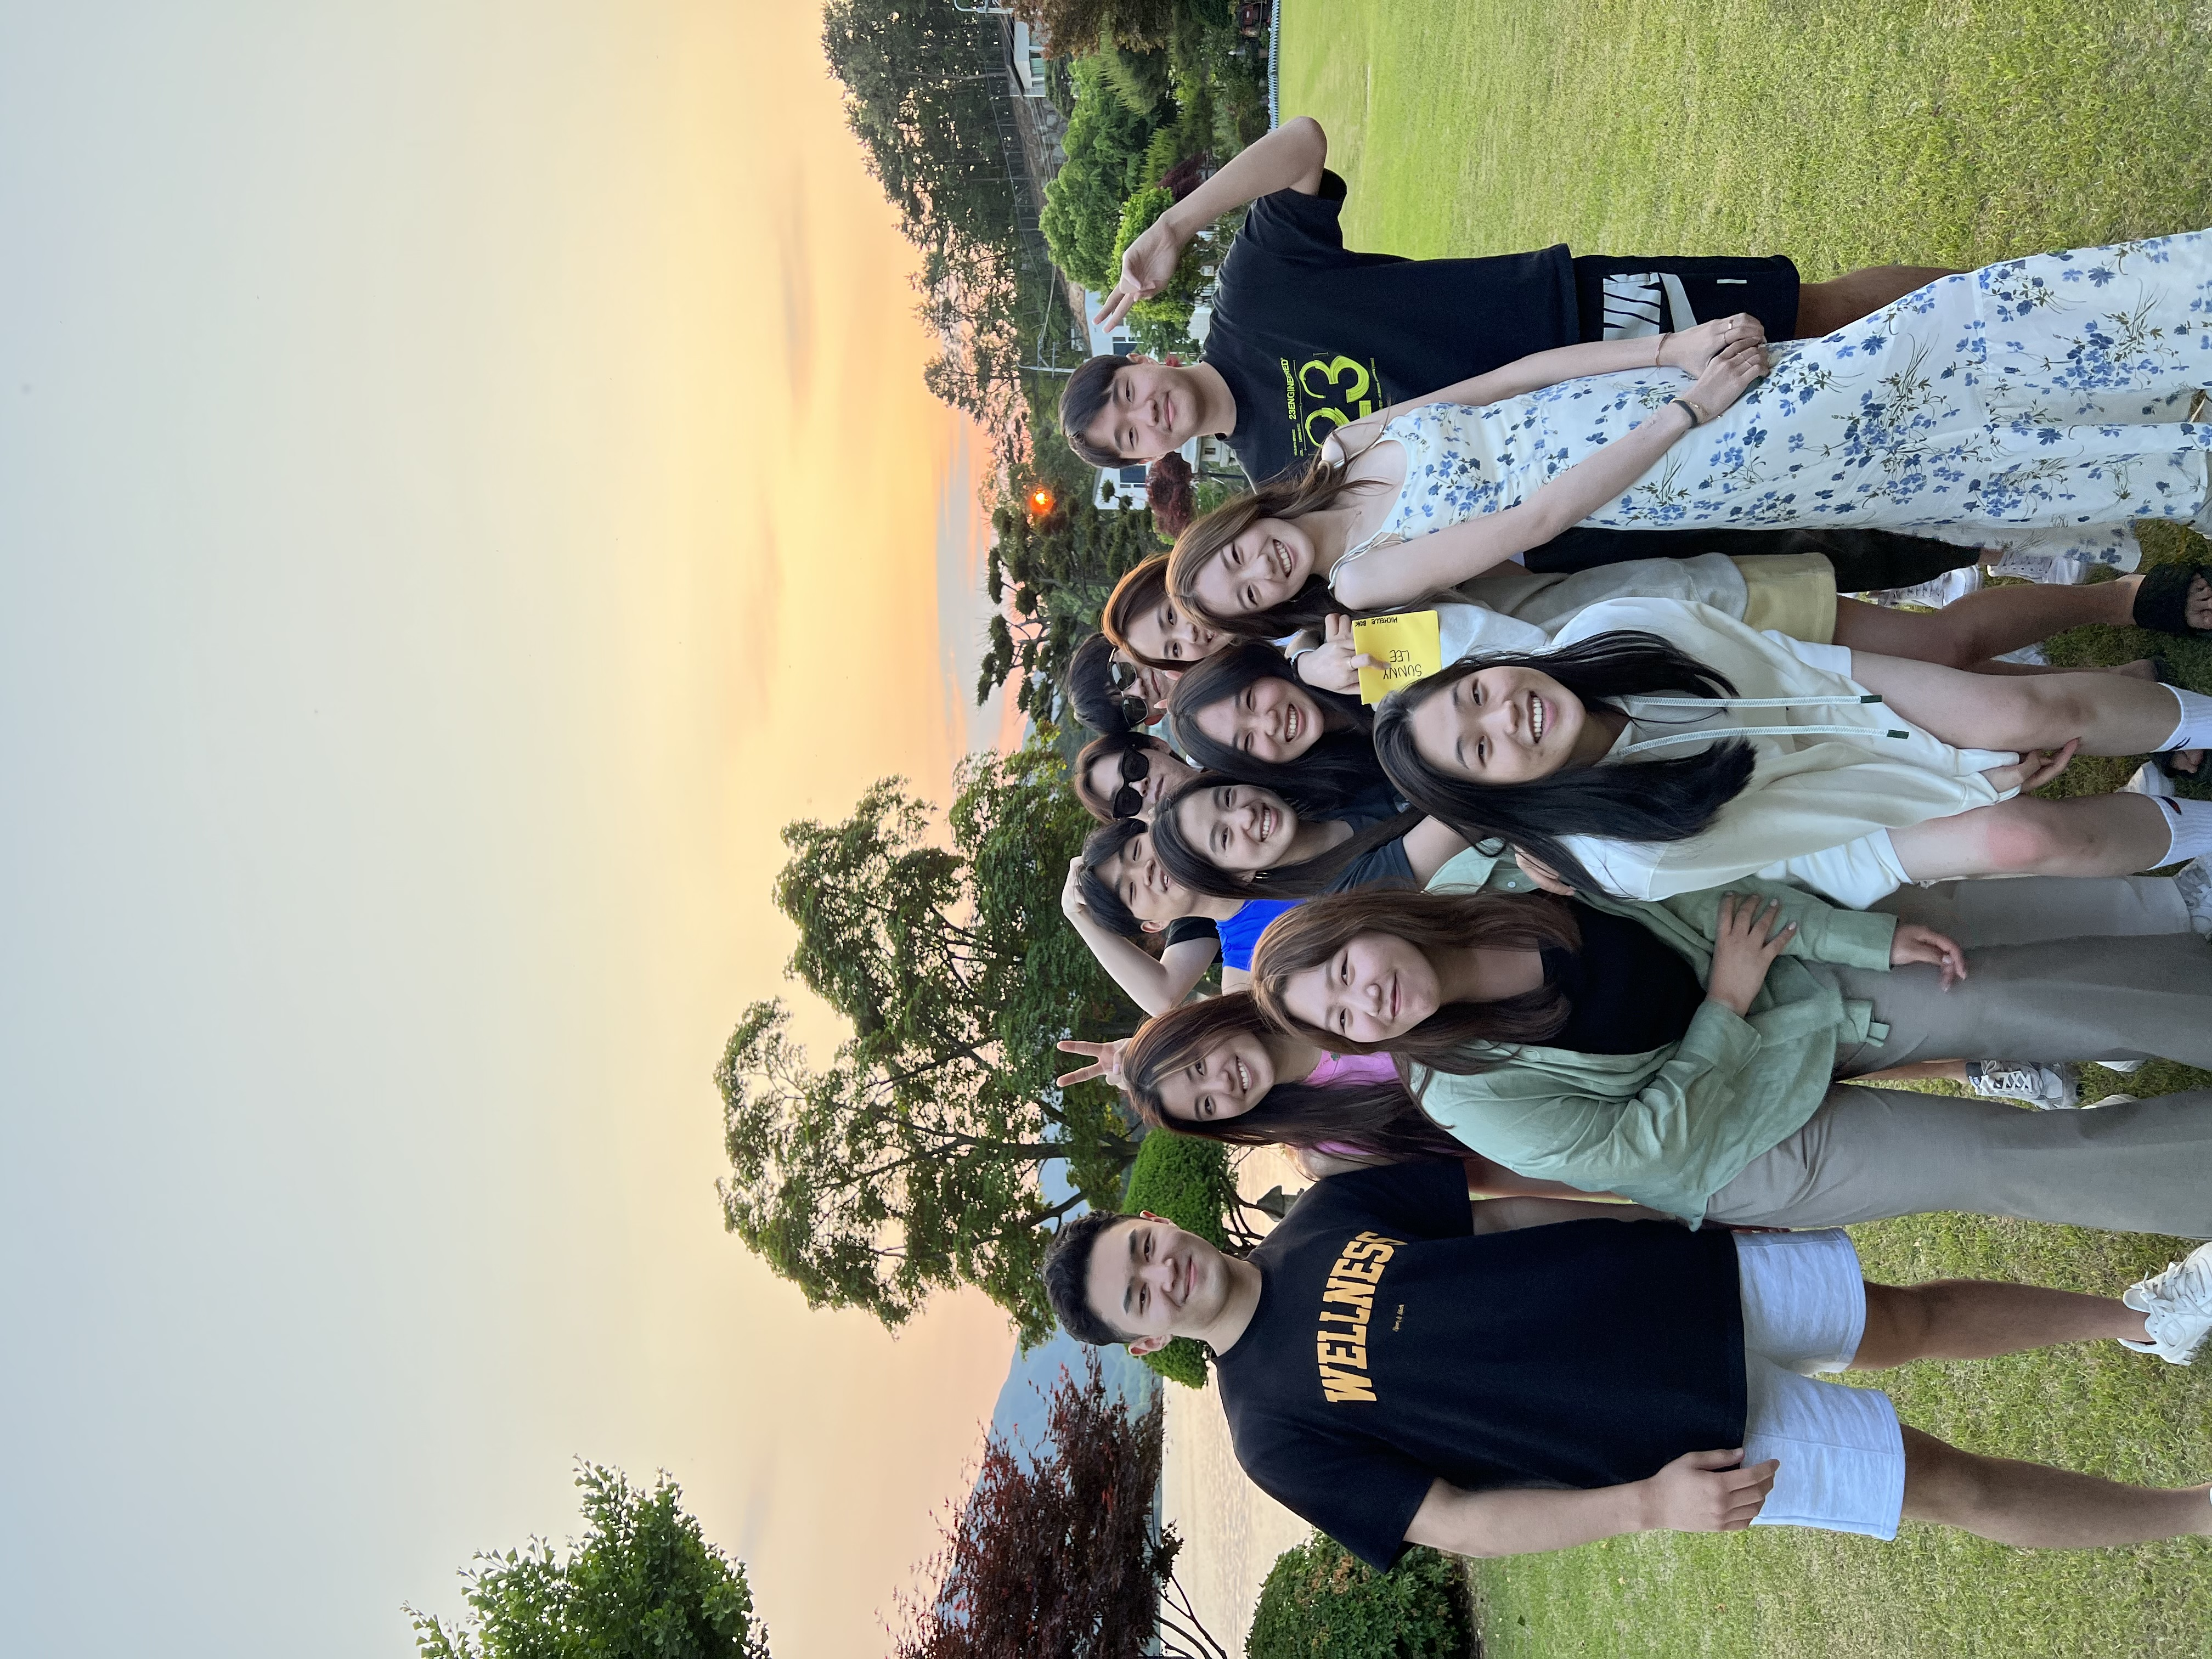
\includegraphics[keepaspectratio]{images/high-school-friends.jpeg}}

}

\caption{High school senior trip with my best friends}

\end{figure}%

\begin{figure}[H]

{\centering \pandocbounded{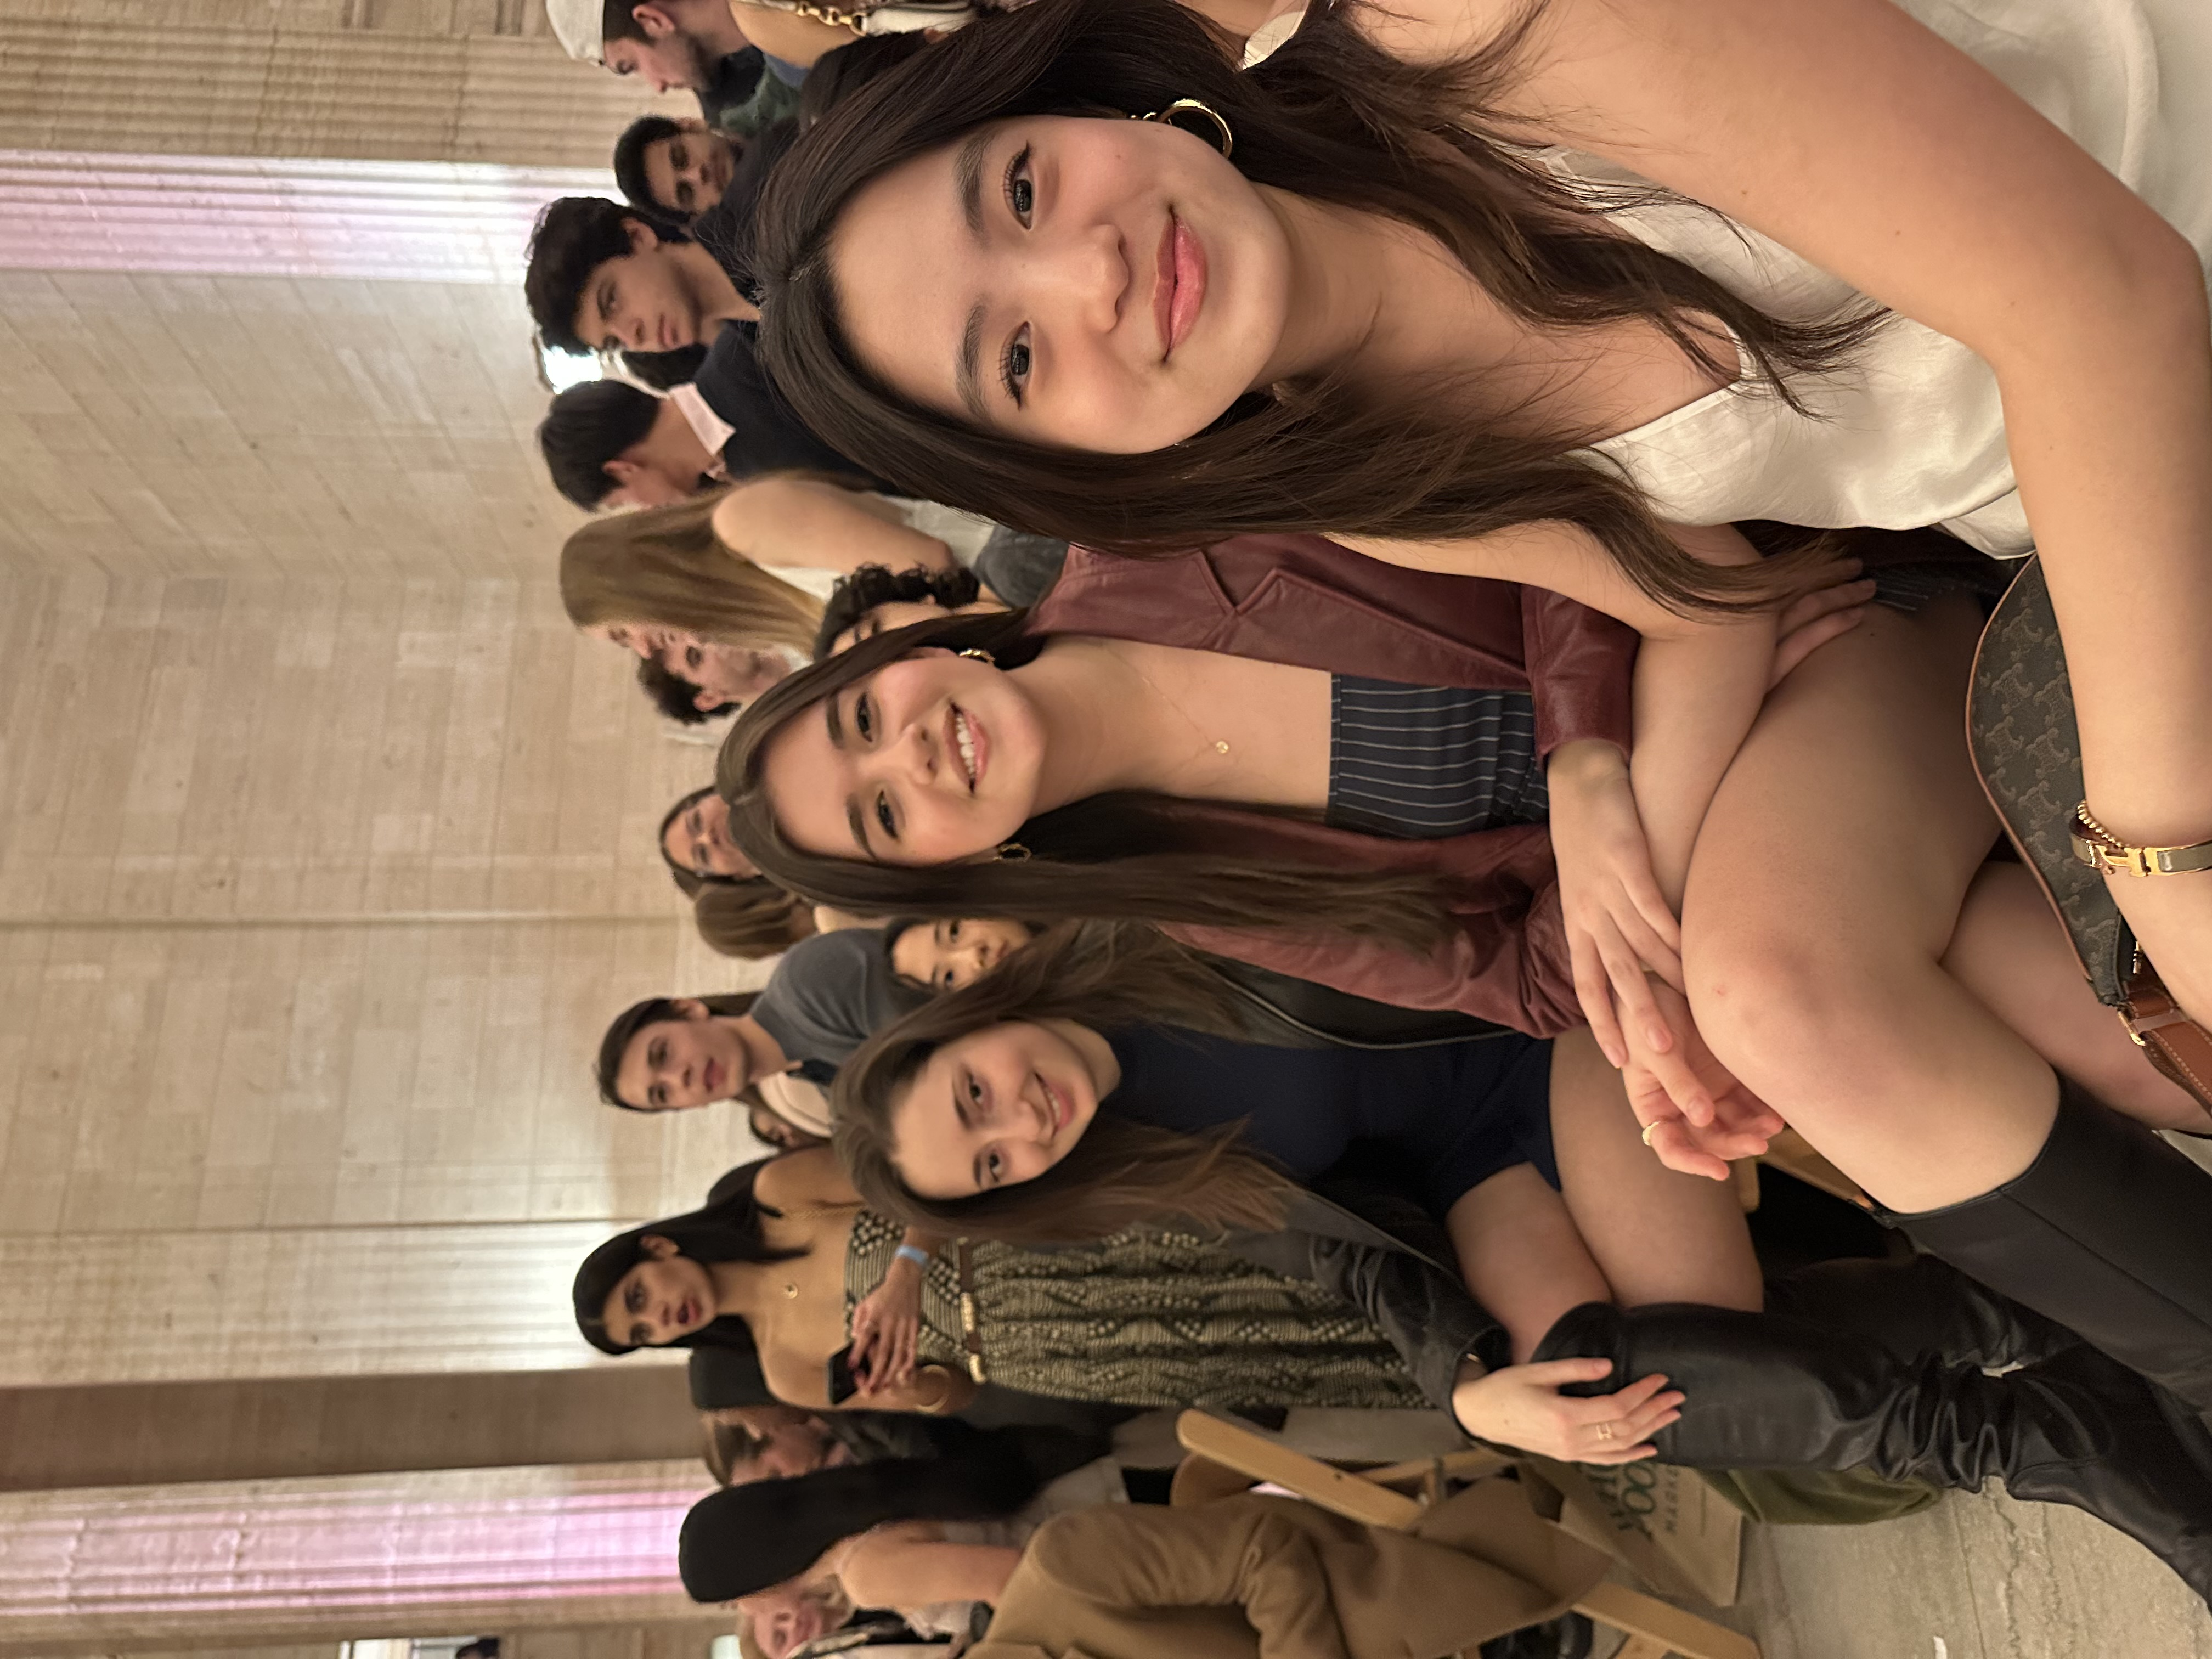
\includegraphics[keepaspectratio]{images/MODA-fashion-show.jpeg}}

}

\caption{At the 2025 MODA Fashion show with my friends}

\end{figure}%

\section{Student Sunny}\label{sec-student-sunny}

I love school. Not that I'm a nerd. But intellectual stimulation is a
core part of my life. It keeps me going. As Bill Gates once said, ``I
don't want my brain to stop working.'' Gates and I have this in common.
My greatest fear is not being able to think. In true Descartes spirit, I
think, therefore I exist or \emph{cogito ergo sum}.

I go to the University of Chicago, and I am a pre-med student majoring
in Biology and Comparative Human Development.

\begin{figure}[H]

{\centering \pandocbounded{\includegraphics[keepaspectratio]{images/uchicago-walk.jpeg}}

}

\caption{UChicago orientation}

\end{figure}%

Confused what a \textbf{comparative human development} major is? You can
find out here:

\href{https://humdev.uchicago.edu/}{Department of Comparative Human
Development}

\subsection{Some of my research work with
R}\label{some-of-my-research-work-with-r}

For example, my research passion is the \textbf{social determinants of
health}. I made a quick example of how my research would look like to
showcase the type of career path I want to go into.

\subsubsection{Brief description and methodology of research
project}\label{brief-description-and-methodology-of-research-project}

My research project involves utilizing a publicly available Medical
Expenditure Panel Survey (MEPS) database to extract relevant variables
and find the relationship between them through statistical analyses. For
example, in the 2021 Full Year Consolidated file in MEPS, there are
variables that measure the social determinants of health, perceived
mental health, and demographic information such as sex and race.

Out of the numerous variables, I make a new database with only the
variables of interest using R. In this mini research project I am able
to showcase, I only included social determinants of health factors that
measure an individual's social support.

Here are the variables I used: ``DUPERSID'', ``SDCHURCH'', ``SDCOMM'',
``SDCOMPAN'', ``SDFAMILY'', ``SDFRIENDS'', ``SDGETTGT'', ``MNHLTH31'',
``SEX'', ``RACETHX''.

The name of ``MNHTLH31'' was changed to ``Perceived\_Mental\_Health'' to
make it more intuitive in my dataframe, and I added a new column
``Social\_Support\_Sum'' that takes all SDOH variables and sums up the
numbers into the column. The less the number, the less social support
they have.

To explore more about data collection method and genreal decription of
MEPS, click here: \href{data/h233doc.pdf}{2021 Consolidated Full Year
File document}

To learn more about the variables, click here:
\href{data/h233cb.pdf}{2021 Consolidated Full Year File codebook}

\subsubsection{Research using R}\label{research-using-r}

Here is how my RStudio screen would look like.

\begin{Shaded}
\begin{Highlighting}[]
\CommentTok{\#|label: source{-}Rscript}

\CommentTok{\# Source R script including data information}
\FunctionTok{source}\NormalTok{(}\StringTok{"student{-}sunny{-}data.R"}\NormalTok{)}
\end{Highlighting}
\end{Shaded}

\begin{verbatim}

Attaching package: 'dplyr'
\end{verbatim}

\begin{verbatim}
The following objects are masked from 'package:stats':

    filter, lag
\end{verbatim}

\begin{verbatim}
The following objects are masked from 'package:base':

    intersect, setdiff, setequal, union
\end{verbatim}

\begin{verbatim}
-- Attaching core tidyverse packages ------------------------ tidyverse 2.0.0 --
v forcats   1.0.0     v stringr   1.5.1
v ggplot2   3.5.1     v tibble    3.2.1
v lubridate 1.9.4     v tidyr     1.3.1
v purrr     1.0.2     
-- Conflicts ------------------------------------------ tidyverse_conflicts() --
x dplyr::filter() masks stats::filter()
x dplyr::lag()    masks stats::lag()
i Use the conflicted package (<http://conflicted.r-lib.org/>) to force all conflicts to become errors

Attaching package: 'scales'


The following object is masked from 'package:purrr':

    discard


The following object is masked from 'package:readr':

    col_factor



Attaching package: 'psych'


The following objects are masked from 'package:scales':

    alpha, rescale


The following objects are masked from 'package:ggplot2':

    %+%, alpha


Loading required package: Matrix


Attaching package: 'Matrix'


The following objects are masked from 'package:tidyr':

    expand, pack, unpack



Attaching package: 'kableExtra'


The following object is masked from 'package:dplyr':

    group_rows


Suggested APA citation: Thériault, R. (2023). rempsyc: Convenience functions for psychology. 
Journal of Open Source Software, 8(87), 5466. https://doi.org/10.21105/joss.05466


Attaching package: 'flextable'


The following objects are masked from 'package:kableExtra':

    as_image, footnote


The following object is masked from 'package:purrr':

    compose
\end{verbatim}

\begin{Shaded}
\begin{Highlighting}[]
\CommentTok{\# Produce the table as an APA formatted table with rempsyc}

\NormalTok{h233\_categorized.long }\SpecialCharTok{\%\textgreater{}\%} 
  \FunctionTok{group\_by}\NormalTok{(ivanddv) }\SpecialCharTok{\%\textgreater{}\%} 
  \FunctionTok{summarize}\NormalTok{(}\AttributeTok{mean =} \FunctionTok{mean}\NormalTok{(value),}
         \AttributeTok{median =} \FunctionTok{median}\NormalTok{(value),}
         \AttributeTok{sd =} \FunctionTok{sd}\NormalTok{(value),}
         \AttributeTok{min =} \FunctionTok{min}\NormalTok{(value),}
         \AttributeTok{max =} \FunctionTok{max}\NormalTok{(value),}
         \AttributeTok{range =}\NormalTok{ max}\SpecialCharTok{{-}}\NormalTok{min,}
         \AttributeTok{range =} \FunctionTok{diff}\NormalTok{(}\FunctionTok{range}\NormalTok{(value))}
\NormalTok{  ) }\SpecialCharTok{\%\textgreater{}\%} \FunctionTok{nice\_table}\NormalTok{()}
\end{Highlighting}
\end{Shaded}

\global\setlength{\Oldarrayrulewidth}{\arrayrulewidth}

\global\setlength{\Oldtabcolsep}{\tabcolsep}

\setlength{\tabcolsep}{2pt}

\renewcommand*{\arraystretch}{1.5}



\providecommand{\ascline}[3]{\noalign{\global\arrayrulewidth #1}\arrayrulecolor[HTML]{#2}\cline{#3}}

\begin{longtable}[c]{ccccccc}
\caption{Summary statistics}\tabularnewline




\ascline{0.5pt}{000000}{1-7}

\multicolumn{1}{>{}c}{\textcolor[HTML]{000000}{\fontsize{12}{24}\selectfont{\global\setmainfont{Times New Roman}{ivanddv}}}} & \multicolumn{1}{>{}c}{\textcolor[HTML]{000000}{\fontsize{12}{24}\selectfont{\global\setmainfont{Times New Roman}{mean}}}} & \multicolumn{1}{>{}c}{\textcolor[HTML]{000000}{\fontsize{12}{24}\selectfont{\global\setmainfont{Times New Roman}{median}}}} & \multicolumn{1}{>{}c}{\textcolor[HTML]{000000}{\fontsize{12}{24}\selectfont{\global\setmainfont{Times New Roman}{sd}}}} & \multicolumn{1}{>{}c}{\textcolor[HTML]{000000}{\fontsize{12}{24}\selectfont{\global\setmainfont{Times New Roman}{min}}}} & \multicolumn{1}{>{}c}{\textcolor[HTML]{000000}{\fontsize{12}{24}\selectfont{\global\setmainfont{Times New Roman}{max}}}} & \multicolumn{1}{>{}c}{\textcolor[HTML]{000000}{\fontsize{12}{24}\selectfont{\global\setmainfont{Times New Roman}{range}}}} \\

\ascline{0.5pt}{000000}{1-7}\endfirsthead 

\ascline{0.5pt}{000000}{1-7}

\multicolumn{1}{>{}c}{\textcolor[HTML]{000000}{\fontsize{12}{24}\selectfont{\global\setmainfont{Times New Roman}{ivanddv}}}} & \multicolumn{1}{>{}c}{\textcolor[HTML]{000000}{\fontsize{12}{24}\selectfont{\global\setmainfont{Times New Roman}{mean}}}} & \multicolumn{1}{>{}c}{\textcolor[HTML]{000000}{\fontsize{12}{24}\selectfont{\global\setmainfont{Times New Roman}{median}}}} & \multicolumn{1}{>{}c}{\textcolor[HTML]{000000}{\fontsize{12}{24}\selectfont{\global\setmainfont{Times New Roman}{sd}}}} & \multicolumn{1}{>{}c}{\textcolor[HTML]{000000}{\fontsize{12}{24}\selectfont{\global\setmainfont{Times New Roman}{min}}}} & \multicolumn{1}{>{}c}{\textcolor[HTML]{000000}{\fontsize{12}{24}\selectfont{\global\setmainfont{Times New Roman}{max}}}} & \multicolumn{1}{>{}c}{\textcolor[HTML]{000000}{\fontsize{12}{24}\selectfont{\global\setmainfont{Times New Roman}{range}}}} \\

\ascline{0.5pt}{000000}{1-7}\endhead



\multicolumn{1}{>{}l}{\textcolor[HTML]{000000}{\fontsize{12}{24}\selectfont{\global\setmainfont{Times New Roman}{Perceived\_Mental\_Health}}}} & \multicolumn{1}{>{}c}{\textcolor[HTML]{000000}{\fontsize{12}{24}\selectfont{\global\setmainfont{Times New Roman}{2.08}}}} & \multicolumn{1}{>{}c}{\textcolor[HTML]{000000}{\fontsize{12}{24}\selectfont{\global\setmainfont{Times New Roman}{2.00}}}} & \multicolumn{1}{>{}c}{\textcolor[HTML]{000000}{\fontsize{12}{24}\selectfont{\global\setmainfont{Times New Roman}{1.22}}}} & \multicolumn{1}{>{}c}{\textcolor[HTML]{000000}{\fontsize{12}{24}\selectfont{\global\setmainfont{Times New Roman}{-8.00}}}} & \multicolumn{1}{>{}c}{\textcolor[HTML]{000000}{\fontsize{12}{24}\selectfont{\global\setmainfont{Times New Roman}{5.00}}}} & \multicolumn{1}{>{}c}{\textcolor[HTML]{000000}{\fontsize{12}{24}\selectfont{\global\setmainfont{Times New Roman}{13.00}}}} \\





\multicolumn{1}{>{}l}{\textcolor[HTML]{000000}{\fontsize{12}{24}\selectfont{\global\setmainfont{Times New Roman}{Social\_Support\_Sum}}}} & \multicolumn{1}{>{}c}{\textcolor[HTML]{000000}{\fontsize{12}{24}\selectfont{\global\setmainfont{Times New Roman}{8.36}}}} & \multicolumn{1}{>{}c}{\textcolor[HTML]{000000}{\fontsize{12}{24}\selectfont{\global\setmainfont{Times New Roman}{10.00}}}} & \multicolumn{1}{>{}c}{\textcolor[HTML]{000000}{\fontsize{12}{24}\selectfont{\global\setmainfont{Times New Roman}{6.83}}}} & \multicolumn{1}{>{}c}{\textcolor[HTML]{000000}{\fontsize{12}{24}\selectfont{\global\setmainfont{Times New Roman}{0.00}}}} & \multicolumn{1}{>{}c}{\textcolor[HTML]{000000}{\fontsize{12}{24}\selectfont{\global\setmainfont{Times New Roman}{28.00}}}} & \multicolumn{1}{>{}c}{\textcolor[HTML]{000000}{\fontsize{12}{24}\selectfont{\global\setmainfont{Times New Roman}{28.00}}}} \\

\ascline{0.5pt}{000000}{1-7}



\end{longtable}



\arrayrulecolor[HTML]{000000}

\global\setlength{\arrayrulewidth}{\Oldarrayrulewidth}

\global\setlength{\tabcolsep}{\Oldtabcolsep}

\renewcommand*{\arraystretch}{1}

\subsubsection{Summary, statistics of
samples}\label{summary-statistics-of-samples}

\begin{Shaded}
\begin{Highlighting}[]
\NormalTok{sex\_table }\OtherTok{\textless{}{-}} \FunctionTok{as.data.frame}\NormalTok{(}\FunctionTok{table}\NormalTok{(h233\_categorized}\SpecialCharTok{$}\NormalTok{SEX))}
\FunctionTok{colnames}\NormalTok{(sex\_table) }\OtherTok{\textless{}{-}} \FunctionTok{c}\NormalTok{(}\StringTok{"Sex"}\NormalTok{, }\StringTok{"Count"}\NormalTok{)}
\FunctionTok{print}\NormalTok{(sex\_table, }\AttributeTok{row.names =} \ConstantTok{FALSE}\NormalTok{)}
\end{Highlighting}
\end{Shaded}

\begin{verbatim}
    Sex Count
   Male 13423
 Female 14913
\end{verbatim}

\begin{Shaded}
\begin{Highlighting}[]
\NormalTok{race\_table }\OtherTok{\textless{}{-}} \FunctionTok{as.data.frame}\NormalTok{(}\FunctionTok{table}\NormalTok{(h233\_categorized}\SpecialCharTok{$}\NormalTok{RACETHX))}
\FunctionTok{colnames}\NormalTok{(race\_table) }\OtherTok{\textless{}{-}} \FunctionTok{c}\NormalTok{(}\StringTok{"Race"}\NormalTok{, }\StringTok{"Count"}\NormalTok{)}
\FunctionTok{print}\NormalTok{(race\_table, }\AttributeTok{row.names =} \ConstantTok{FALSE}\NormalTok{)}
\end{Highlighting}
\end{Shaded}

\begin{verbatim}
               Race Count
           Hispanic  6798
 Non-Hispanic White 15023
 Non-Hispanic Black  4071
 Non-Hispanic Asian  1385
 Non-Hispanic Other  1059
\end{verbatim}

\begin{Shaded}
\begin{Highlighting}[]
\CommentTok{\#|label: bar{-}plot}

\CommentTok{\# dplyr package has filter() function}
\FunctionTok{library}\NormalTok{(dplyr)}

\CommentTok{\# Define factor labels}
\NormalTok{mental\_health\_labels }\OtherTok{\textless{}{-}} \FunctionTok{c}\NormalTok{(}\StringTok{"1"} \OtherTok{=} \StringTok{"Excellent"}\NormalTok{, }
                          \StringTok{"2"} \OtherTok{=} \StringTok{"Very Good"}\NormalTok{, }
                          \StringTok{"3"} \OtherTok{=} \StringTok{"Good"}\NormalTok{, }
                          \StringTok{"4"} \OtherTok{=} \StringTok{"Fair"}\NormalTok{, }
                          \StringTok{"5"} \OtherTok{=} \StringTok{"Poor"}\NormalTok{)}

\CommentTok{\# Filter out invalid values and recode as factors}
\NormalTok{h233\_filtered }\OtherTok{\textless{}{-}}\NormalTok{ h233\_categorized }\SpecialCharTok{\%\textgreater{}\%}
  \FunctionTok{filter}\NormalTok{(Perceived\_Mental\_Health }\SpecialCharTok{\%in\%} \DecValTok{1}\SpecialCharTok{:}\DecValTok{5}\NormalTok{) }\SpecialCharTok{\%\textgreater{}\%}
  \FunctionTok{mutate}\NormalTok{(}\AttributeTok{Perceived\_Mental\_Health =} \FunctionTok{factor}\NormalTok{(Perceived\_Mental\_Health, }
                                          \AttributeTok{levels =} \DecValTok{1}\SpecialCharTok{:}\DecValTok{5}\NormalTok{, }
                                          \AttributeTok{labels =}\NormalTok{ mental\_health\_labels))}

\CommentTok{\# Load necessary package to make bar graph}
\FunctionTok{library}\NormalTok{(ggplot2)}

\CommentTok{\# Create the plot}
\FunctionTok{ggplot}\NormalTok{(h233\_filtered, }\FunctionTok{aes}\NormalTok{(}\AttributeTok{x =}\NormalTok{ Perceived\_Mental\_Health)) }\SpecialCharTok{+}
  \FunctionTok{geom\_bar}\NormalTok{() }\SpecialCharTok{+}
  \FunctionTok{labs}\NormalTok{(}\AttributeTok{title =} \StringTok{"Frequency of Perceived Mental Health"}\NormalTok{, }
       \AttributeTok{x =} \StringTok{"Perceived Mental Health Measure"}\NormalTok{, }
       \AttributeTok{y =} \StringTok{"Count"}\NormalTok{, }
       \AttributeTok{caption =} \StringTok{"MNHLTH31 variables used"}\NormalTok{) }\SpecialCharTok{+}
  \FunctionTok{theme\_minimal}\NormalTok{()}
\end{Highlighting}
\end{Shaded}

\pandocbounded{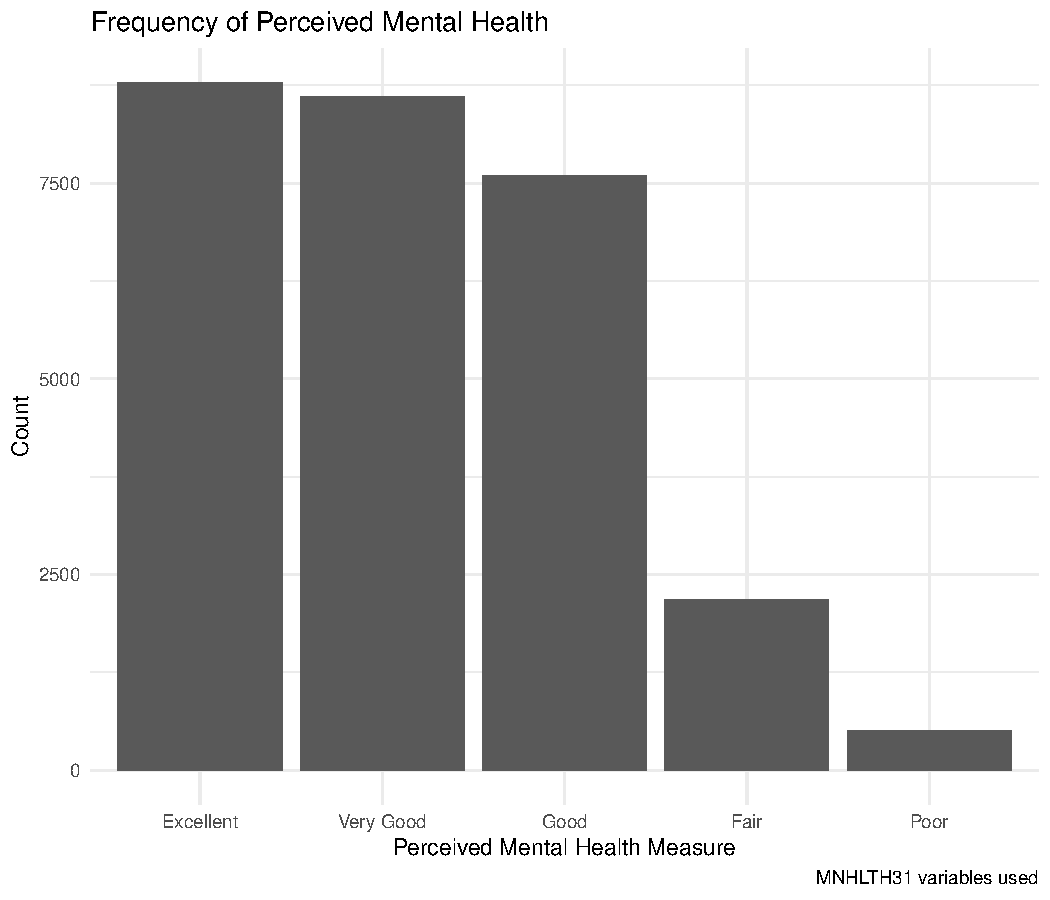
\includegraphics[keepaspectratio]{index_files/figure-pdf/unnamed-chunk-15-1.pdf}}

From this bar graph, we can see that the distribution of perceived
mental health in individuals is more positive than negative.

\subsubsection{Correlation statistics}\label{correlation-statistics}

\section{Other passions and quirks}\label{sec-other}

Yogi, foodie, \#trackstar, dog mom, neat freak, and more




\end{document}
